\documentclass[12pt,a4paper]{article}
% The following LaTeX packages must be installed on your machine: amsmath, authblk, bm, booktabs, caption, dcolumn, fancyhdr, geometry, graphicx, hyperref, latexsym, natbib
\input{183.dat}
\usepackage{gensymb}
\usepackage{amsthm}
\usepackage{float}
\usepackage{siunitx}
\usepackage{amssymb}
\usepackage{float}
\usepackage{enumerate}
\usepackage{listings}
\usepackage{mathtools}
\PassOptionsToPackage{hyphens}{url}\usepackage{hyperref}
\usepackage[none]{hyphenat}
\usepackage{physics}
\newcommand\ddfrac[2]{\frac{\displaystyle #1}{\displaystyle #2}}
%\renewcommand{\familydefault}{\sfdefault}


\begin{document}

\setcounter{page}{1}

\section*{LE3 Problem 2}
\bigskip

\begin{enumerate}[a)]

\item \textbf{Sketch of output}

\begin{figure}[h!]
	\centering
	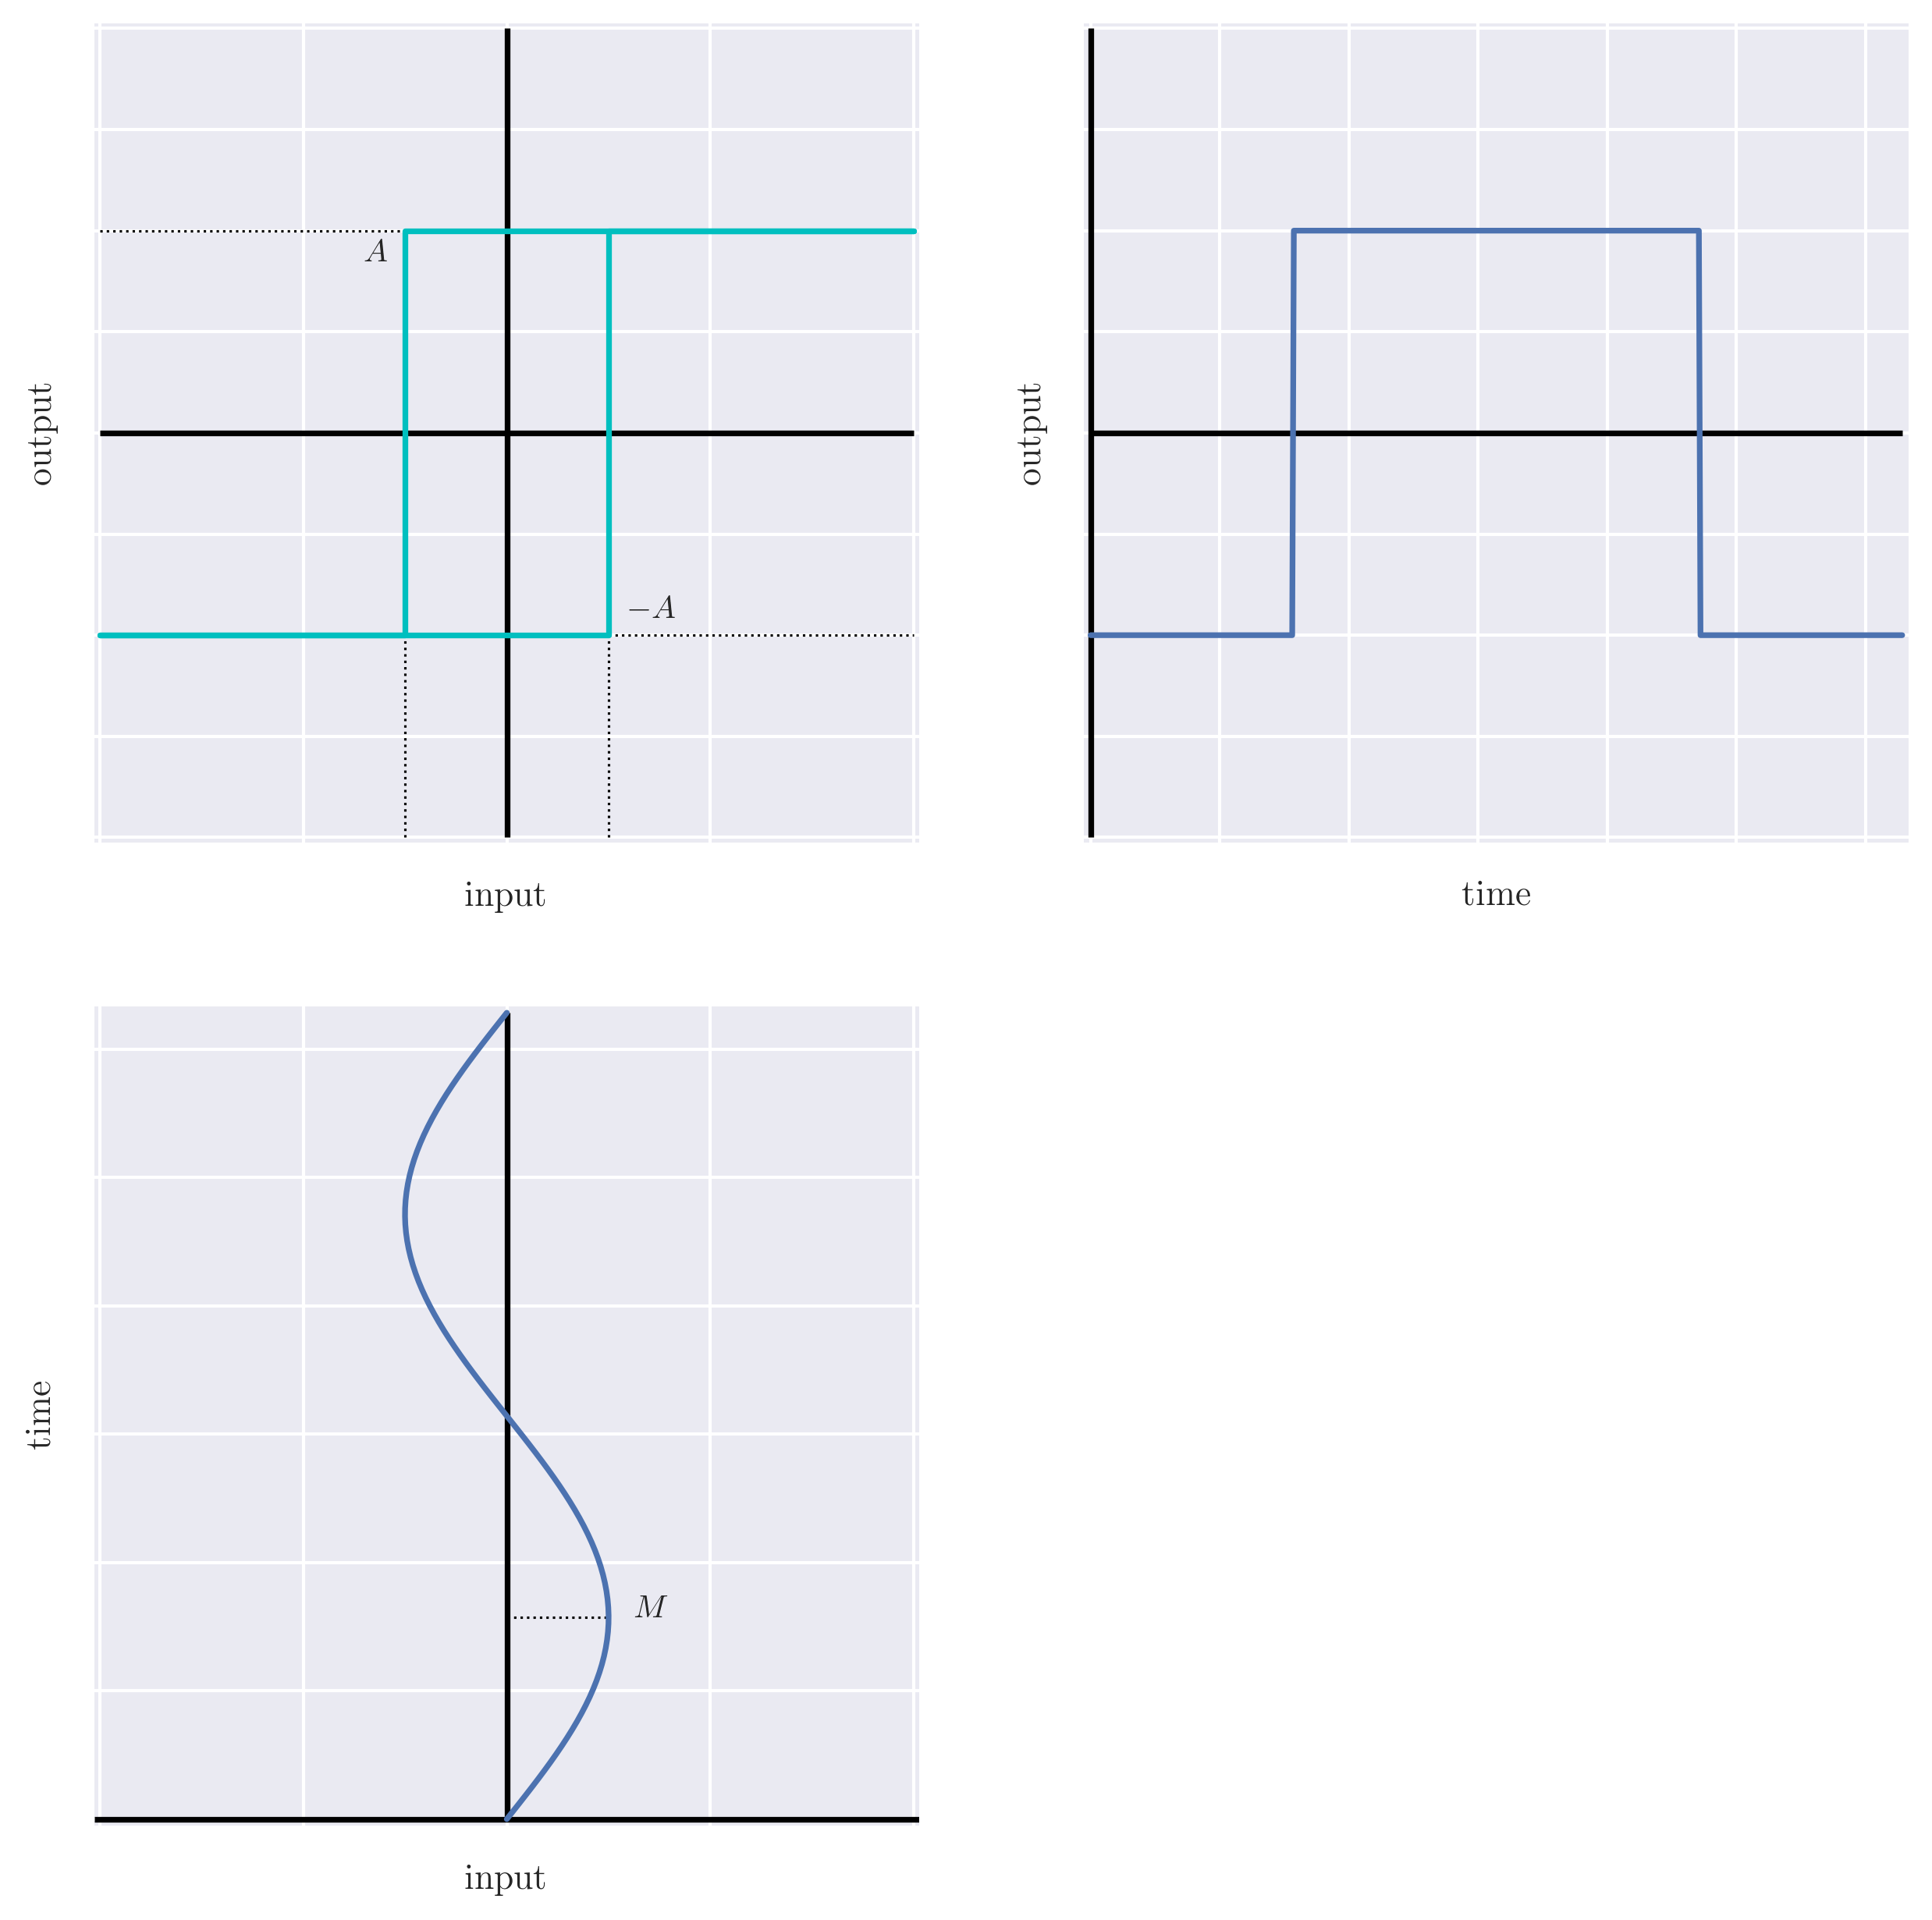
\includegraphics[width=\linewidth]{LE3_io.png}
	\caption{IO curves of an ideal relay with hysteresis, with a sinusoidal input.}
	\label{fig:desc-hysteresis}
\end{figure}

Consider an input of the form $M\sin(\omega t)$ being controlled by an ideal relay with hysteresis. The output for one cycle of the input can be described as

\begin{equation}
	n(t) =
	\begin{cases}
		-A & , \quad 0 \leq t \leq \frac{\pi}{2} \\
		A & , \quad \frac{\pi}{2} < t \leq \frac{3\pi}{2} \\
		-A & , \quad \frac{3\pi}{2} < t \leq T
	\end{cases} \label{eq:output}
\end{equation}

\item \textbf{Fourier coefficients}

We cascade $n(t)$ with some linear system $G(s)$, which we take in this case to be a low-pass filter, and equate it to the first-order terms of the Fourier series:

\begin{equation}
	n(t) = A_1 \cos(\omega t) + B_1 \sin(\omega t)
\end{equation}

Figs. \ref{fig:prod-ncos} and \ref{fig:prod-nsin} show the product of $n(t)$ with $\cos(\omega t)$ and $\sin(\omega t)$, respectively.

\begin{figure}[h!]
	\centering
	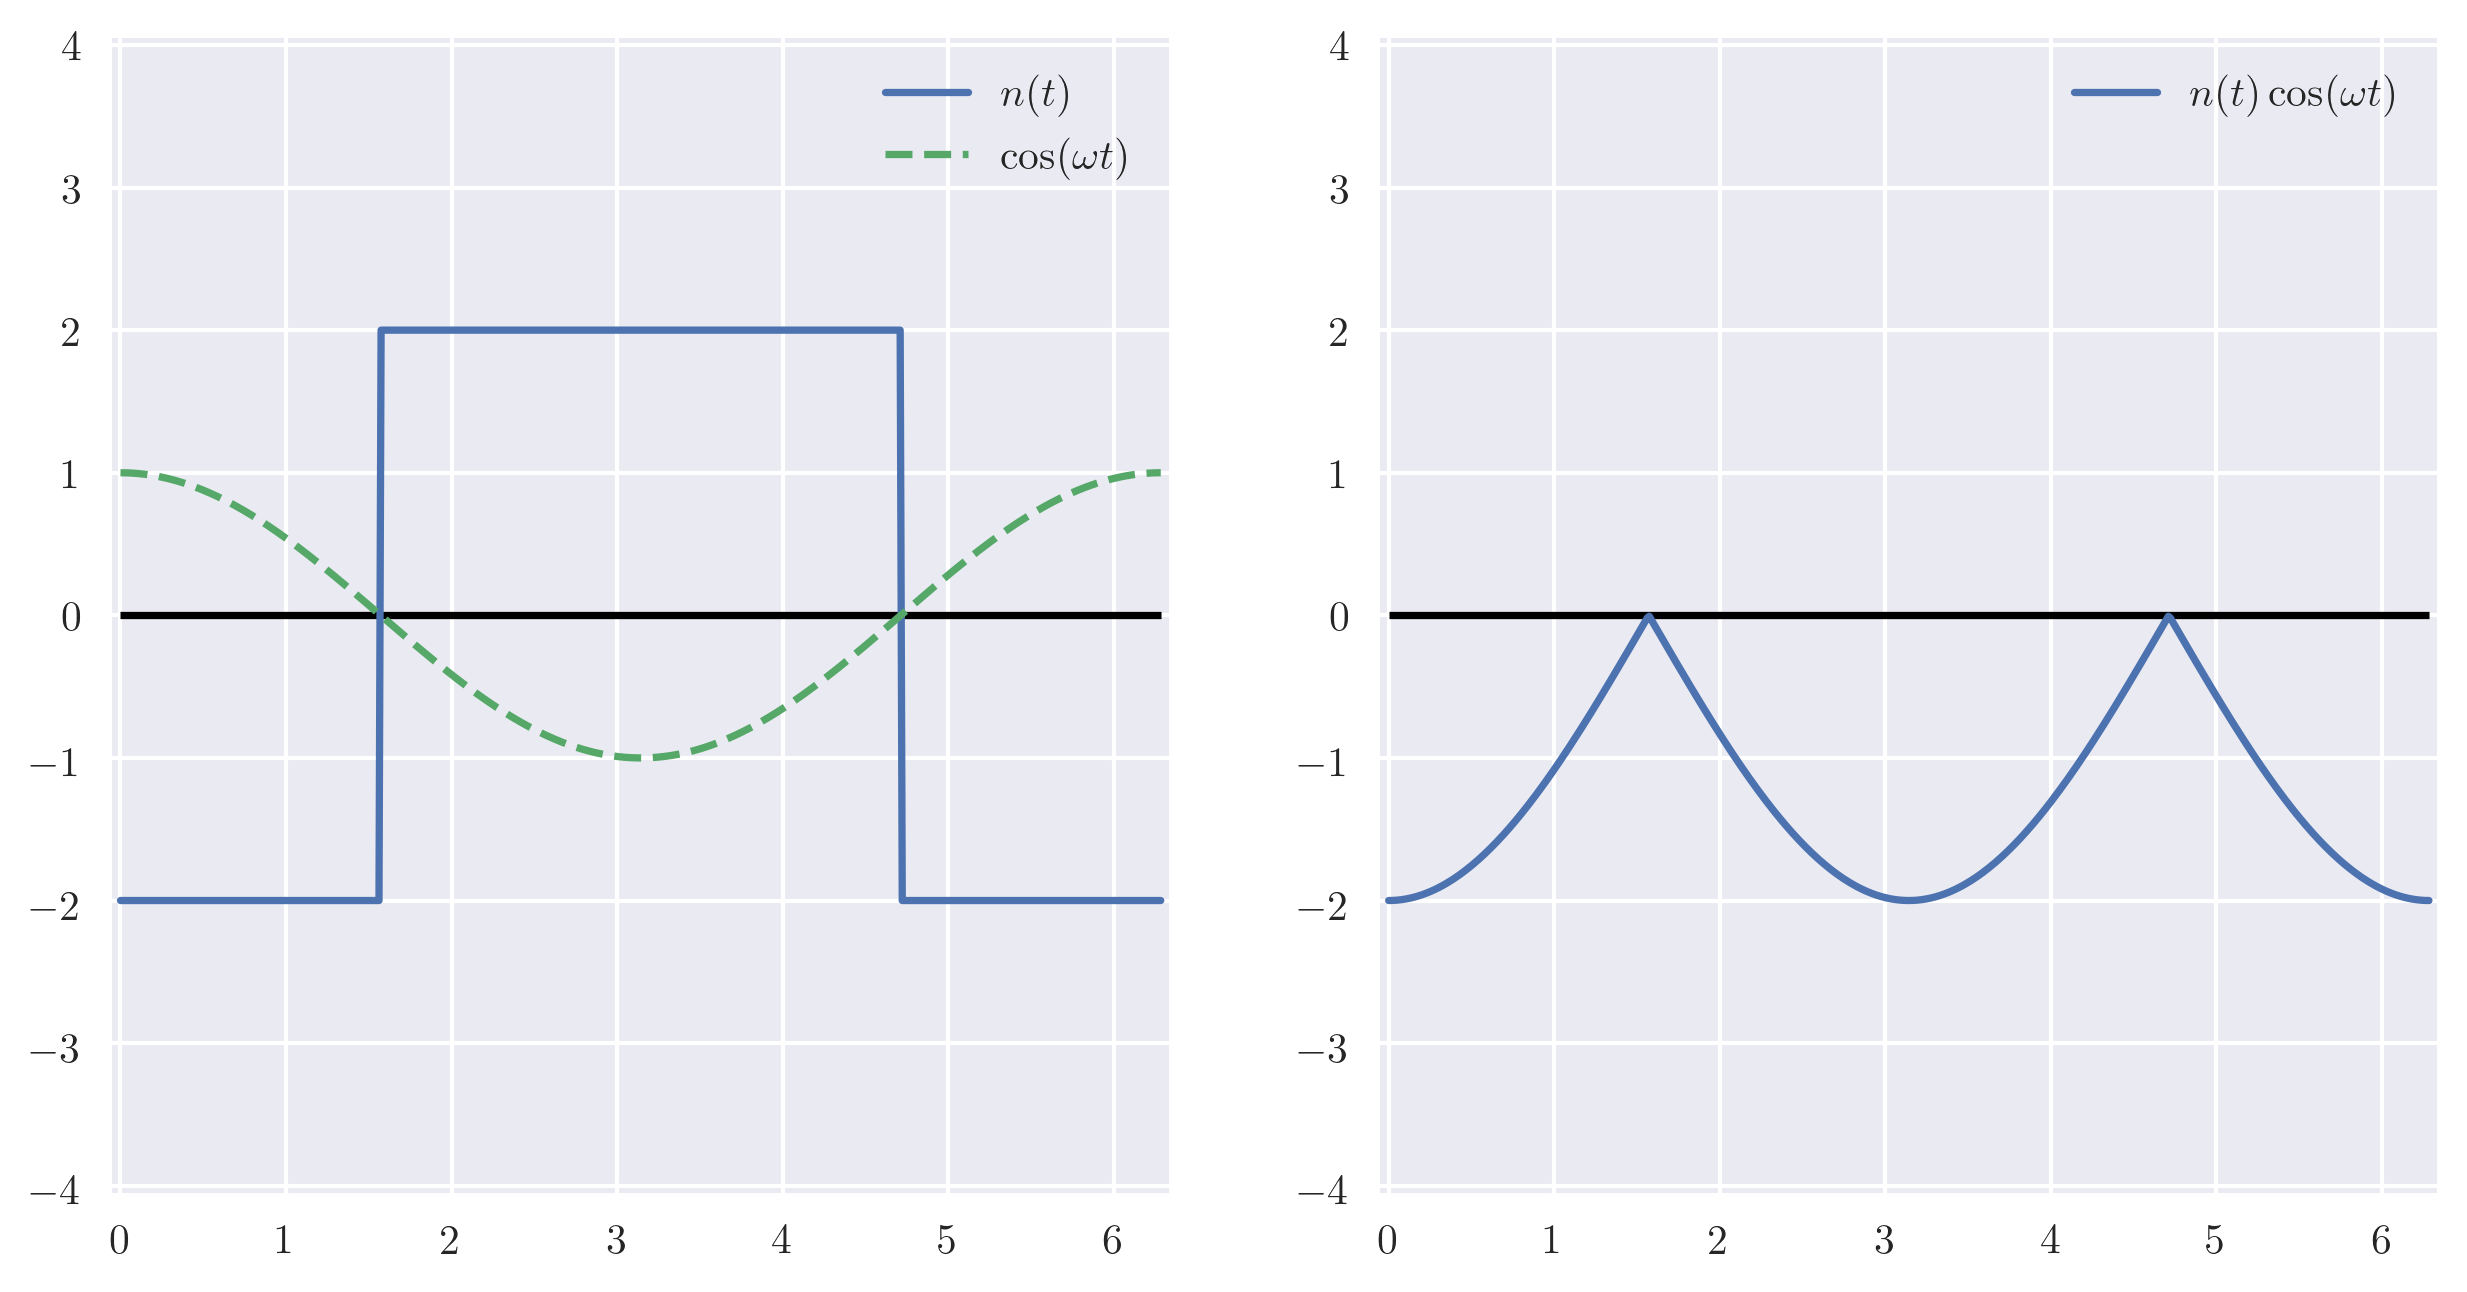
\includegraphics[width=\linewidth]{LE3_prod-ncos.png}
	\caption{Product of $n(t)$ and $\cos(\omega t)$, with $\abs{M} = 1$, $\abs{A} = 2$.}
	\label{fig:prod-ncos}
\end{figure}

\begin{figure}[h!]
	\centering
	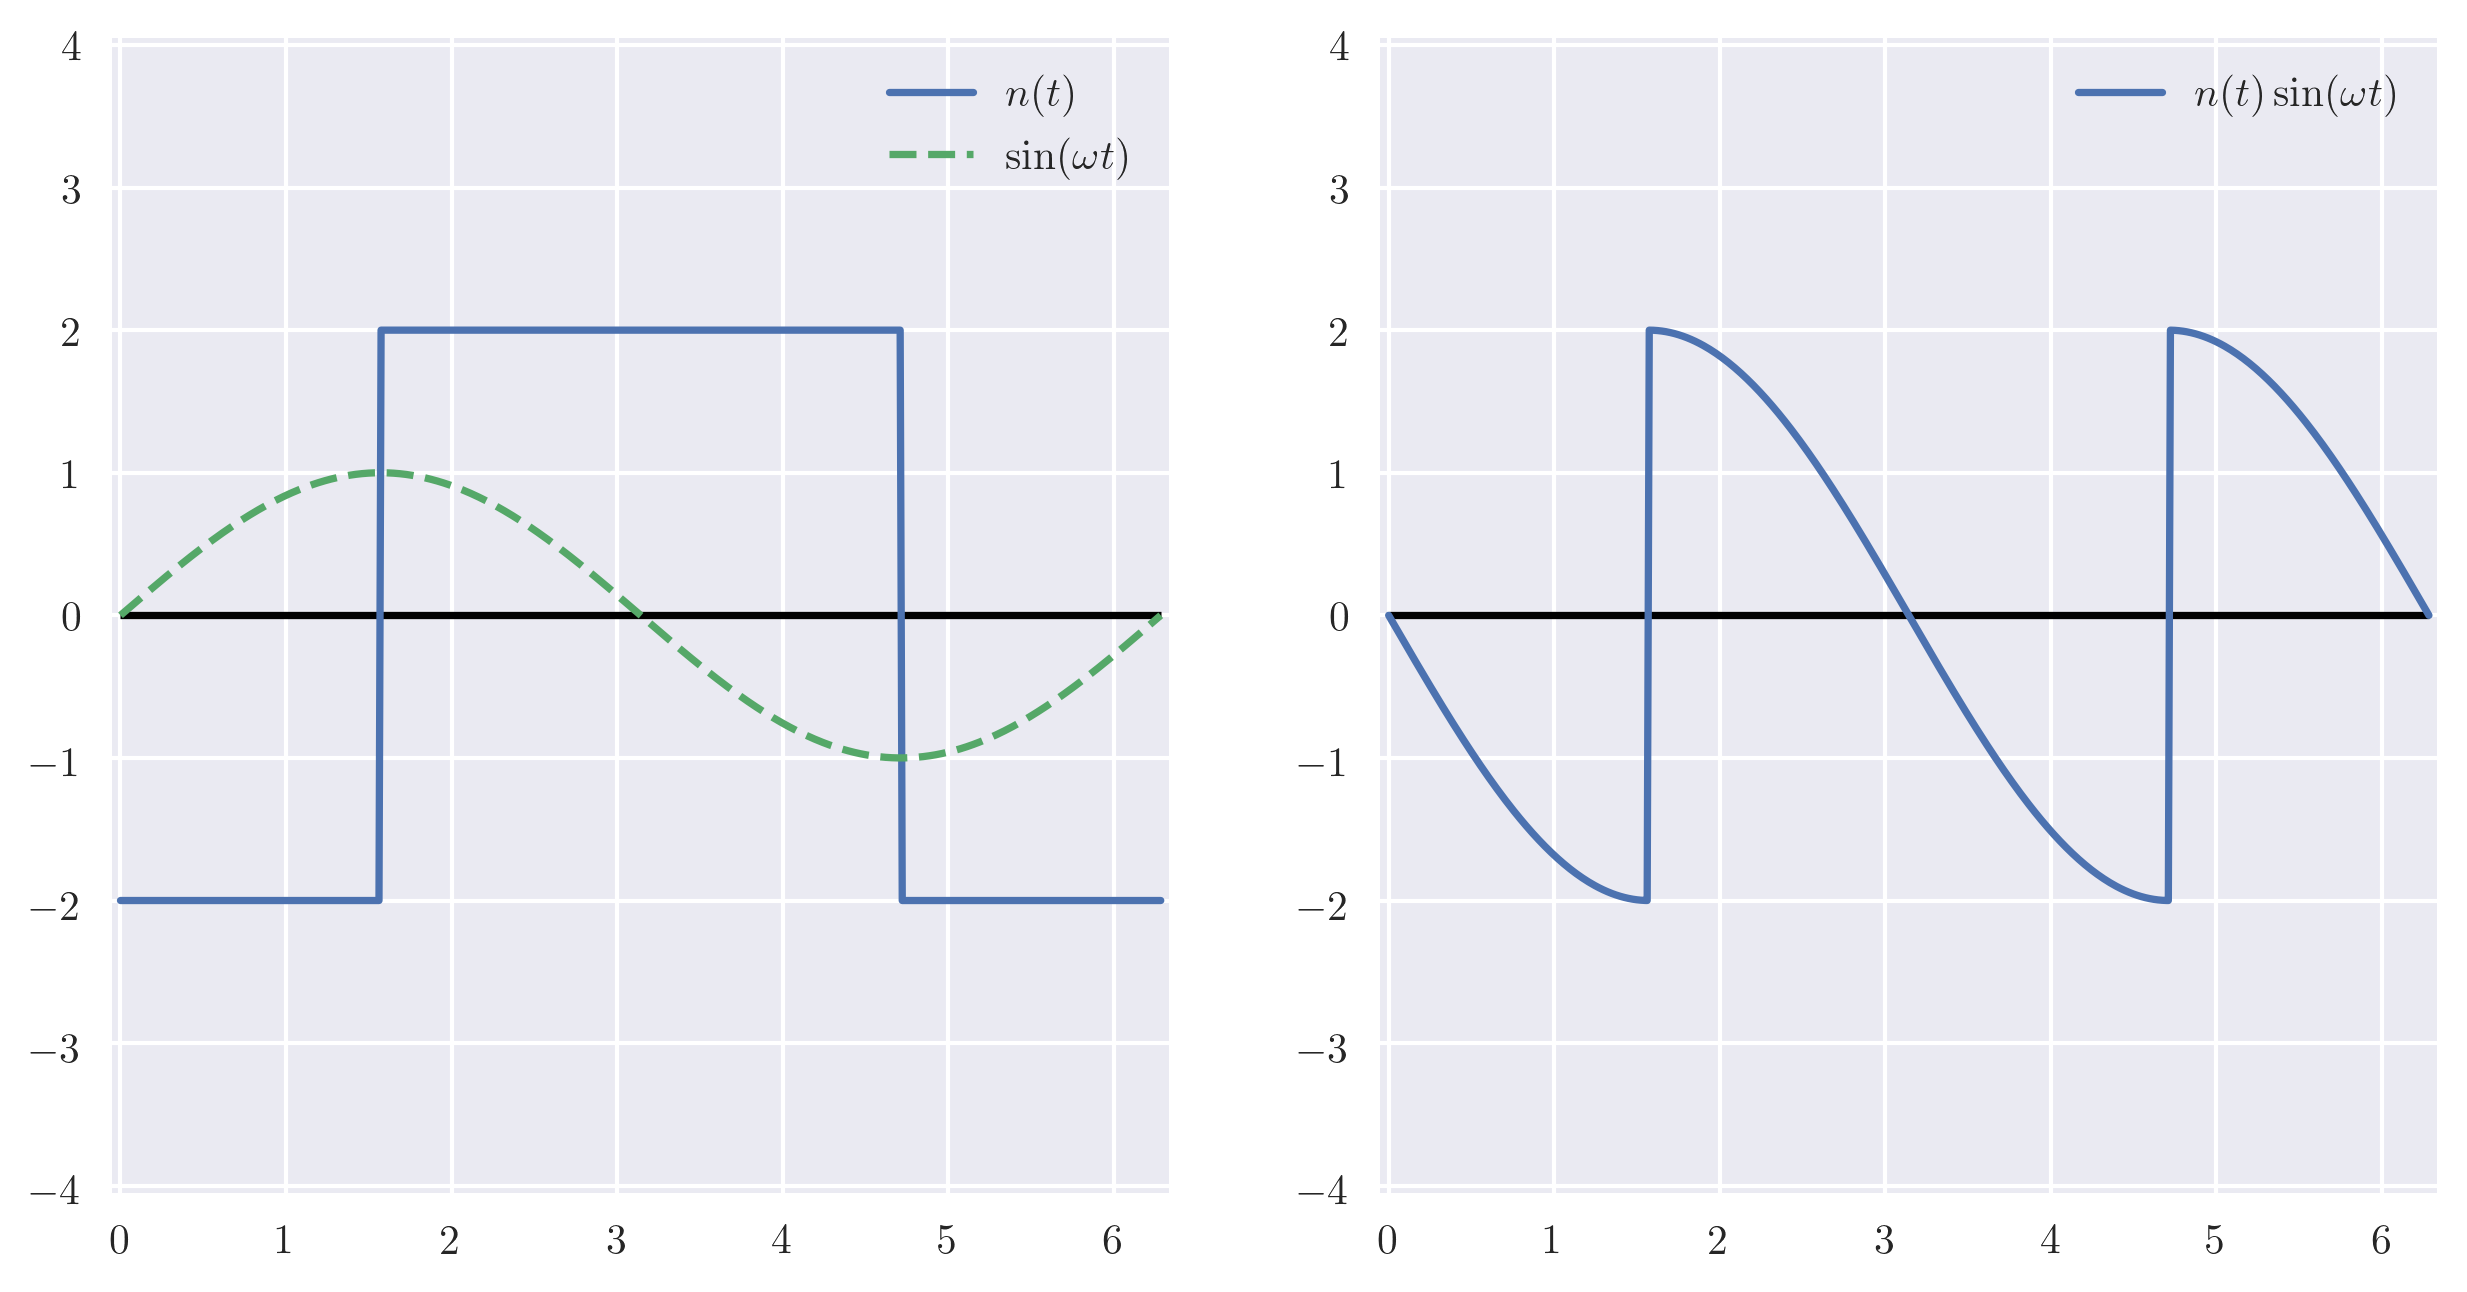
\includegraphics[width=\linewidth]{LE3_prod-nsin.png}
	\caption{Product of $n(t)$ and $\sin(\omega t)$, with $\abs{M} = 1$, $\abs{A} = 2$.}
	\label{fig:prod-nsin}
\end{figure}

By graphical analysis, we see that the output is even when multiplied by $\cos$, and odd when multiplied by $\sin$. Therefore, the integral of the $\sin$ term vanishes and $\boxed{B_1 = 0}$. Letting $T \equiv 2\pi/\omega$ (one wave period), the coefficient $A_1$ can be calculated by

\begin{equation}
	A_1 = \frac{2}{T} \int_{t_0}^{t_0 + T} n(t)\cos(\omega t) \dd{t}
\end{equation}

For simplicity, we take $t_0 = 0$ and integrate w.r.t. $\omega t$ over one cycle s.t. $T = 2\pi$. Evaluating $A_1$:

\begin{align}
	A_1 &= \frac{1}{\pi} \int_0^{2\pi} n(t)\cos(\omega t)\dd{(\omega t)} \\
	&= \frac{1}{\pi} \qty[\int_0^{\pi/2} -A\cos(\omega t) \dd{(\omega t)} + \int_{\pi/2}^{3\pi/2} A\cos(\omega t) \dd{(\omega t)} + \int_{3\pi/2}^{2\pi} -A\cos(\omega t) \dd{(\omega t)}] \\
	&= \frac{A}{\pi} \qty[\int_0^{\pi/2} -\cos(\omega t) \dd{(\omega t)} + \int_{\pi/2}^{3\pi/2} \cos(\omega t) \dd{(\omega t)} + \int_{3\pi/2}^{2\pi} -\cos(\omega t) \dd{(\omega t)}] \\
	&= \frac{A}{\pi} \qty[-\eval{\sin(\omega t)}_{\omega t = 0}^{\pi/2} + \eval{\sin(\omega t)}_{\omega t = \pi/2}^{3\pi/2} - \eval{\sin(\omega t)}_{\omega t = 3\pi/2}^{2\pi}] \\
	&= \frac{A}{\pi} \qty[-1 - 2 - 1] \\
	\Aboxed{
		A_1 &= -\frac{4A}{\pi}
	} \label{eq:A1}
\end{align}

\item \textbf{Describing function}

The describing function is calculated as:

\begin{align}
	N(M, \omega) &= \frac{B_1 + jA_1}{M} \\
	&= -\frac{jA_1}{M} \\
	\Aboxed{
		N(M, \omega) &= -\frac{4jA}{\pi M}
	} \label{eq:N}
\end{align}

\end{enumerate}

\end{document}